%=== CHAPTER TWO (2) ===
%=== Literature Review ===

% TODO: Add the .bib references so that they are listed properly.

\chapter{Literature Review}
\begin{spacing}{2.0}
	%\setlength{\parskip}{0.2in}

	\section{Chapter Introduction}

	Video games are constantly evolving to provide more engaging and immersive experiences to players, be it by improved graphics fidelity, better story telling, or by increasing the challenge.
	When it comes to the balancing difficulty to player skill, traditional difficulty techniques often fail to properly adapt to the vast range of player skill levels, and the difference on how fast certain players learn.
	Dynamic Difficulty Adjustment (DDA), along with Reinforcement Learning (RL) agents emerge as solutions to adapt game difficulty in real time based on player performance, along with decreasing predictability and
	increasing the challenge players face, enhancing player immersion, motivation and increasing replayability \cite{grech_creating_2023} \cite{mercieca_evaluating_2023} \cite{attard_analysing_2021}. This section explores and discusses previous works and their results regarding DDA and RL agents in video games
	to identify the current state of the art and to provide a foundation for the research conducted in this thesis.

	% make dda come after Unity-ML.
	\section{Dynamic Difficulty Adjustment (DDA)}

	Dynamic Difficulty Adjustment (DDA) refers to a game design approach where a set of systems dynamically alter the difficulty of a game through modifying game parameters such as AI behaviour,
	player and enemy stats, or environmental factors in real time to match player's skill. These systems target maintaining player engagement to be in line with Csikszentmihalyi's Flow Model, also known as the
	"flow state", a mental condition that is characterised by its ability to keep players deeply immersed and focus on gameplay, avoiding boredom or frustration \cite{grech_creating_2023} \cite{mifsud_utilizing_2021} \cite{laus_dynamic_2022} \cite{vang_impact_2022}.

	% Mention the flow state a bit more
	\begin{figure}[ht]
		\centering
		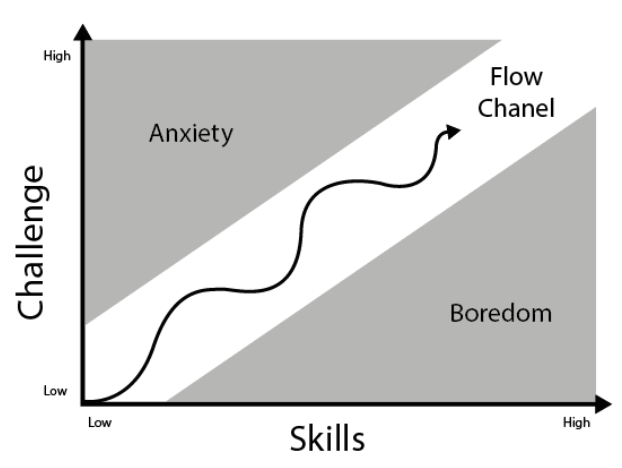
\includegraphics[width=5in, fbox]{Figures/Flow_State.png}
		\caption{Flow State. \cite{sepulveda_exploring_2019}}
		\label{fig:flowstate}
	\end{figure}

	One of the fundamental aspects of DDA is its adaptability to player performance, which allows it to better accomodate the diverse range of player skill levels and learning speeds, avoiding the frustration that
	can occur with traditional fixed difficulty settings. Research has shown that several DDA implementations, such as ramping (rDDA) and player-controlled adjustments (pDDA), can significantly improve player experience.
	And recently, these approaches on DDA have been combined with AI techniques and algorithms to create more sophisticated and responsive systems that can adapt to player performance in real time, such as
	Deep Reinforcement Learning (DRL), Fuzzy Logic, Decision trees and Monte Carlo Tree Search (MCTS) \cite{attard_analysing_2021} \cite{chrysafiadi_fuzzy_based_2023}.
	% Mention the specific data needed for DDA to work in these types of games \cite{grech_creating_2023}

	\subsection{Determining Player Skill}

	Determining player skill is a crucial aspect of DDA, as if the DDA system is innaccurate, it can lead to the opposite effect, where the player will become more bored or frustrated, and can even lead to player's
	leaving the game. To develop effective DDA systems, it is crucial that developers take care to choose the variables that best determine the player's skill level. In the work done by Hunicke {31}, the Hamlet DDA system was used to
	closely monitor the core inventory, including the players health, shielding, ammunition, and weapons, adjusting the difficulty of the level based on the player's items. In a combat encounter, the DDA system was
	developed to see rapid depletion of items as a sign of player struggle, and therefore the system would intervene by modifying the level to aid the player {31}.

	\section{Static Game Difficulties}

	Currently, most games use static difficulty settings, where players choose a static difficulty level before starting the game.
	There are many reasons for this, such as the simplicity of implementation, the ability to control the player experience
	and progression, and that in the past players did not like the instability of dynamic difficulty systems, which with older algorithms
	did not have access nor the ability to process the complex data needed for DDA to work in these types of games \cite{attard_analysing_2021}

	\subsection{Fixed Difficulties}

	These fixed difficulties rely on pre-set levels (e.g., easy, medium, hard) chosen by players before playing, and suffer from
	being rigid and unable to adapt to player performance, skill levels or evolving gameplay dynamics \cite{attard_analysing_2021} \cite{laus_dynamic_2022}.
	% Discuss more

	\subsection{Difficulty Selection}

	With difficulty selection, players can change the difficulty during gameplay, helping in reducing the frustration or boredom that
	comes from fixed difficulties, and helps in keeping players engaged for longer periods \cite{attard_analysing_2021} \cite{laus_dynamic_2022}. However, this approach still requires players to manually adjust the difficulty,
	which can be cumbersome and disrupt the flow of the game, and are still rigid in nature, leading to the difficulty always being either too easy or too hard \cite{attard_analysing_2021} \cite{laus_dynamic_2022}.
	% Discuss more

	\section{Dynamic Difficulty Adjustment Compared with Static Difficulties}

	As discussed, dynamic systems outperform static ones when it comes to keeping to Csikszentmihalyi's Flow Model, helping reduce player boredom and frustration while enhancing both player immersion and replayability,
	thus keeping players engaged for longer periods \cite{grech_creating_2023} \cite{attard_analysing_2021} \cite{mifsud_utilizing_2021}. The main drawbacks of DDA come from its more complex development process, the need for more data and computational resources, and the potential for it to
	become more boring and frustrating than fixed difficulties if not implemented correctly, and given an adequate amount of real-time data \cite{attard_analysing_2021} \cite{laus_dynamic_2022}.

	\subsection{Game Immersion and replayability}

	Studies such as those done by \cite{mercieca_evaluating_2023} \cite{attard_analysing_2021} \cite{mifsud_utilizing_2021} \cite{laus_dynamic_2022} \cite{vang_impact_2022} confirm that DDA significantly improves player immersion by keeping players in a balanced challenge zone, keeping them both motivated and better entertained, resulting in
	a better player experience. Furthermore, the dynamic nature of these systems motivate players to revisit games, as the change in difficulty and challenges they present the player scale with the player's skill,
	keeping the game feeling fresh and engaging where fixed difficulties could not \cite{grech_creating_2023} \cite{attard_analysing_2021} \cite{mifsud_utilizing_2021} \cite{laus_dynamic_2022} \cite{sepulveda_exploring_2019}.

	\section{AI with DDA Algorithms}

	Studies have also shown that in recent time, AI has played a pivotal role in improving on the implementation of DDA systems by allowing better decision making and data processing based on player performance metrics.
	Such models are Reinforcement Learning (RL), as shown in the work done by \cite{mercieca_evaluating_2023} \cite{mifsud_utilizing_2021} \cite{zheng_dynamic_2024}, fuzzy logic \cite{chrysafiadi_fuzzy_based_2023}, Monte Carlo Tree Search (MCTS) \cite{demediuk_monte_2017} \cite{soemers_enhancements_2016}, and Decision Trees \cite{sejrsgaard_jacobsen_dynamic_2011}, also known as Behaviour trees.
	These different AI algorithms have helped enable more nuanced and responsive DDA implementations, offering players what feels like a more tailored experience \cite{attard_analysing_2021} \cite{vodopivec_monte_2017} \cite{chrysafiadi_fuzzy_based_2023}.

	\section{Adaptive Gameplay AI Algorithms}

	\subsection{Deep Reinforcement Learning (DRL) Algorithm}

	% TODO: Go more in depths about PPO, since it is the most common algorithm used in games.
	RL algorithms, and in turn Deep Reinforcement Learning (DRL) algorithms use neural networks to enable AI agents to learn and adapt to the situation presented to them. This is done through multiple methods, with the
	most common being Proximal Policy Optimisation (PPO), the State Action Reward State Action (SARSA) and Q-learning algorithms, which have been used to great effect in games like \cite{bin_ramlan_implementation_2021} \cite{metz_evaluation_2020}. They work by placing the agent in a controlled environment,
	where they learn through trial and error, being rewarded for good decisions and penalised for poor ones. This causes the agent to learn the optimal strategy for the situation presented to them,
	and can be used not only as opponents or allies in games, but also as a way to dynamically adjust game difficulty in real time, particularly in fighting games and other high-interaction environments,
	as seen in the works done by \cite{mercieca_evaluating_2023} \cite{mifsud_utilizing_2021} \cite{zheng_dynamic_2024}.
	% Discuss these works a lot more in the RL Agents section, which will be moved above this.

	% Mention the flow state a bit more
	\begin{figure}[ht]
		\centering
		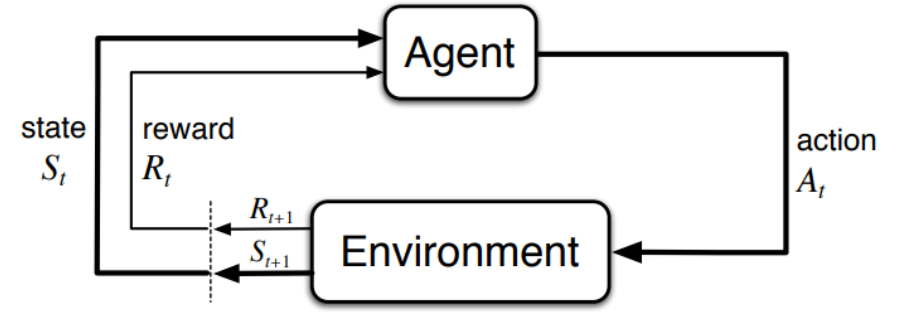
\includegraphics[width=5in, fbox]{Figures/SarSa.png}
		\caption{Agent training environment interaction in RL. \cite{grech_creating_2023}}
		\label{fig:rl_training}
	\end{figure}

	% Should likely expand, but only once the latter part about RL-Agents is done. On top of that, too much time has been spent fine tuning this, and as such it is likely better to move on to the other sections and then come back to it.
	% Q-Learning and Proximal Policy Optimisation (PPO) algorithms, which have been used to
	% Algorithms such as Proximal Policy Optimization (PPO) have been effective in tailoring game difficulty in real time, particularly in fighting games and other high-interaction environments \cite{bin_ramlan_implementation_2021} \cite{metz_evaluation_2020}.

	\subsection{Fuzzy Logic}

	In the study done by Chrysafiadi, et al. \cite{chrysafiadi_fuzzy_based_2023}, Fuzzy logic systems were employed to dynamically adjust game difficulty to match the player's skill level, with the goal of maintaining player engagement while teaching them HTML programming.
	Fuzzy logic systems are particularly effective in such real-time adjustments, as they require less training data when compared to ML models. Moreover, trhese systems offer immediate real-time adjustments to better align with player performance.
	The results of this study show that player dropouts decreased significantly, and player engagement and motivation increased, and even performed better than other groups, proving that fuzzy-based DDA can enhance
	educational outcomes and help keep players in the Flow State with reduced data \cite{chrysafiadi_fuzzy_based_2023}.
	% Perhaps add statistics and more information on the study?

	\subsection{Monte Carlo Tree Search (MCTS)}

	MCTS works by exploring different game states in the form of simulations to optimise decision-making, and is done by building a search tree iteratively, balancing exploration and exploitation to find the best
	move \cite{vodopivec_monte_2017} \cite{demediuk_monte_2017}. In the work done by Demediuk, et al. \cite{demediuk_monte_2017}, MCTS was used to enhance player engagement by modifying AI strategies to maintain balanced matches, with variants like Reactive Outcome-Sensitive Action Selection (ROSAS).
	ROSAS is reactive in nature, which can make it feel unnatural, whilst Proactive OSAS (POSAS), which is more proactive and can feel more natural, at the cost of precision. In the work done by Soemers, et al. \cite{soemers_enhancements_2016},
	different MCTS optimisations were made, such as Progressive History (PH) and N-Gram Selection Technique (NST), where PH biases the selection step towards actions that have been successful in the past, and NST
	biases the play-out step towards actions that have been successful in the past, with the results showing that when combined these greatly improve the algorithm's performance. Another improvement was Deteministic
	Game Detection (DGD), which modifies MCTS behaviour to optimise for deterministic games by using alternative evaluation strategies, which was effective when combined with other enhancements \cite{soemers_enhancements_2016}.
	What these studies show, is that when it comes to more complex and deterministic games, MCTS can be a powerful tool to enhance player engagement both as an opponent, as well as a tool to dynamically adjust
	game difficulty.

	\subsection{Decision \& Behaviour Trees}

	% TODO: Split Decision and behaviour trees based on extra research done.
	Decision trees are popular tools in data analysis, and are used for classification and prediction due to their intuitive structure, which include nodes (root, internal, leaf) and branches \cite{song_decision_2015} \cite{mienye_survey_2024}.
	The framework around how decision trees work when it comes to games varies, as not only can it reduce code repetition in game development, both for complex and simple games \cite{vuong_artificial_2020}, but its structure allows for easy
	interpretation and visualisation of the algorithm's decision making process, making them particularly useful for adapting game features dynamically, as seen in the work done by \cite{sejrsgaard_jacobsen_dynamic_2011}.
	Their approach involved examining two distinct approaches, one using predefined behaviour trees of varying difficulties, and another employing a single tree with dynamic adjustment of probabilities to alter difficulty.
	The first approach struggled when it came to flexibility, as it could not adapt to player performance, which was in stark contrast with the second approach, which was able to optimise behaviour probabilities
	and display superior adaptability, helping to keep the player in the Flow State, and maintain player engagement \cite{sejrsgaard_jacobsen_dynamic_2011}. Along with this, decision trees have been shown to be even more effective when combined with
	other algorithms, such as RL, which help greatly in improving their efficiency and scalability in complex gaming environments, or even with state machines in more simple environments \cite{mcquillan_survey_nodate} \cite{sejrsgaard_jacobsen_dynamic_2011}.

	% Here

	\section{Procedural Content Generation}

	Procedural Content Generation (PCG) is a technique used in game development to create game content algorithmically, leveraging algorithms to dynamically create and add content such as levels, environments,
	and items to games that both help in reducing development time and costs, but also increase replayability and can easily be combined with DDA systems to create more engaging and immersive experiences \cite{laus_dynamic_2022}.
	When paired not only with DDA, but also with AI agents, such as those created by \cite{grech_creating_2023}, PCG was used to constantly modify the best possible action that the player and the agent could take, which in turn
	not only forced the player to adapt to the changing environent, but also helped keep the player feeling challenged and engaged, avoiding frustration since the opponent was also having to adapt in a human like way,
	helping in keeping the player in the Flow State.
	% This needs to be cut down and made better

	% Should finite state machines be included here?

	\section{Unity ML-Agents and how they work}

	Unity ML Agents is a toolkit that enables developers to more easily create and integrate intelligent agents within Unity environments using Machine Learning (ML) techniques.
	The package allows users to transform any scene into a training enviroment where agents can be trained using algorithms such as RL, Imitation Learning and neuroevolution, by allowing agents to observe their surroundings, take actions and receive rewards,
	as well as specifying the behaviours that these agents can take \cite{raut_unity_2024} \cite{unity_ml_agents}.

	\subsection{Finite State Machines}

	Traditionally, and even to this day the most common way to implement AI in games is through Finite State Machines (FSM), which are used to describe a relationship between a set of states, where transitions
	between these states are determined by condition, with actions being performed based on the current state \cite{grech_creating_2023}. FSMs are useful in simple environments, however as the number of actions and states are limited, However
	as the number of states increase, so does the complexity of the FSM, making it difficult to manage, debug and maintain \cite{grech_creating_2023}.

	\subsection{RL Agents}

	As mentioned in an earlier section, RL agents are AI agents that learn through trial and error, being rewarded for good decisions and penalised for poor ones. RL-Agents trained using Unity ML-Agents have more
	access to the environment and its data, and this has been used in the work done by Grech \cite{grech_creating_2023}, where he trained an RL-Agent to act as an opponent in a Real Time Strategy (RTS) game, taking multiple stages of the agent
	in training for the different difficulties. There were also different RL-Agent models such as the Proximal Policy Optimisation (PPO) and others that were used to act as enemies in fighting games \cite{bin_ramlan_implementation_2021}, bosses \cite{metz_evaluation_2020},
	and even for racing games \cite{berta_development_2024}. In these works, along with those done by \cite{borg_investigating_2020} \cite{zhasulanov_enhancing_2024} \cite{raut_unity_2024}, it was revealed that RL-Agents have shown many times to be an effective way to make a more unpredictable, life-like and challenging
	opponent for player, significantly boosting their experience and engagement.

	\subsection{RL Agents compared with Finite State Machines}

	The main differences between FSMs and RL-Agents are their development time and costs, as FSM's are easier and cheaper to implement, but are then limited in their complexity and scalability, where as RL-Agents
	take more time and resources to develop, but solve the issues with FSMs being their complexity, scalability, and the simple fact that when a player fights an FSM enough, they will learn the patterns and states,
	making the game predictable and boring \cite{grech_creating_2023} \cite{bin_ramlan_implementation_2021} \cite{metz_evaluation_2020}. This life-like aspect to RL-Agents can, and have been shown to greatly improve game replayability and immersion, keeping the player in the flow state for longer
	and providing a superior experience to the player \cite{grech_creating_2023} \cite{bin_ramlan_implementation_2021} \cite{metz_evaluation_2020}. With all of this however, it is important to not that if an RL-Agent is not implemented or trained correctly, it can lead to the opposite effect,
	where an opponent is too difficult, leading to player frustration, or too easy, leading to player boredom \cite{grech_creating_2023} \cite{bin_ramlan_implementation_2021} \cite{metz_evaluation_2020}.

	\subsection{Practical Applications}

	As mentioned in the previous sections, RL-Agents have been used in a variety of games, from RTS games to fighting games and now even racing games. The practical applications of RL-Agents in games are vast,
	and as hardware capabilities improve, and our understanding and training techniques improve, the potential for RL-Agents in games is almost limitless. The ability to create more engaging, immersive and challenging
	opponents for players, as well as allies, and the ability to easily integrate them with DDA systems, PCG and other game development techniques to make games more replayable and engaging is a powerful tool for developers
	to create better games \cite{grech_creating_2023} \cite{borg_investigating_2020} \cite{zhasulanov_enhancing_2024} \cite{raut_unity_2024} \cite{metz_evaluation_2020}

	\section{Chapter Overview}

	This chapter has provided an overview on the current state of the art in Dynamic Difficulty Adjustment (DDA) and Reinforcement Learning (RL) agents in video games, and how individually they have been used to
	improve upon more static techniques, such as fixed difficulties and Finite State Machines (FSMs). It has shown that integrating AI techniques has helped in improving the accuracy and adaptability of DDA systems,
	and the latest advancements in RL-Agents, including the Unity ML-Agents package, have shown just how revolutionary these techniques are at improving player engagement and immersion, as well as game replayability
	when these techniques are implemented.
	% Should more sources be referenced since this is more of a summary of the chapter?

	% TODO: Some parts have not been added to this from the word document, and some information is currently missing, however too much time has been spent on this draft so it is best to move on to the next section
	% and wait for feedback and then come back to this section to make the necessary changes.
	% On top of that, due to there being too much information not being condensed properly, the analysis is not as deep as it should be, and this should be improved in the next draft following recommendations.

	%=== END OF CHAPTER TWO ===
\end{spacing}
\newpage
